\section{Empirical Results}

\subsection{Descriptive Properties}
\begin{table}[!htbp]
\centering
\caption{Summary statistics of daily log returns.}
\label{tab:summary-statistics}
\begin{tabular}{lrrrrr}
\toprule
ETF & Mean & Std. Dev. & Skewness & Kurtosis & ACF(1) \\
\midrule
ECH & -0.00002 & 0.01733 & -0.624 & 10.600 & -0.012 \\
EWW & 0.00016 & 0.01597 & -1.068 & 9.448 & -0.010 \\
EWZ & 0.00018 & 0.02365 & -1.137 & 13.272 & -0.133 \\
GXG & -0.00020 & 0.01725 & -1.214 & 16.423 & 0.146 \\
\bottomrule
\end{tabular}
\end{table}

\begin{table}[!htbp]
\centering
\caption{Stationarity and serial dependence diagnostics.}
\label{tab:diagnostics}
\begin{tabular}{lrrrr}
\toprule
ETF & ADF p (price) & ADF p (return) & LB p (return) & LB p (return$^2$) \\
\midrule
ECH & 0.348 & 0.000 & 0.000 & 0.000 \\
EWW & 0.805 & 0.000 & 0.000 & 0.000 \\
EWZ & 0.094 & 0.000 & 0.000 & 0.000 \\
GXG & 0.050 & 0.000 & 0.000 & 0.000 \\
\bottomrule
\end{tabular}
\caption*{\footnotesize ADF is Augmented Dickey-Fuller test; LB is Ljung-Box at lag 10.}
\end{table}

\begin{table}[!htbp]
\centering
\caption{Pairwise correlation matrix of daily log returns.}
\label{tab:return-correlations}
\begin{tabular}{lrrrr}
\toprule
ETF & ECH & EWW & EWZ & GXG \\
\midrule
ECH & 1.000 & 0.586 & 0.568 & 0.581 \\
EWW & 0.586 & 1.000 & 0.662 & 0.611 \\
EWZ & 0.568 & 0.662 & 1.000 & 0.578 \\
GXG & 0.581 & 0.611 & 0.578 & 1.000 \\
\bottomrule
\end{tabular}
\end{table}


\Cref{tab:summary-statistics} shows near-zero unconditional mean returns with heavy tails. \Cref{tab:diagnostics} confirms stationary returns, mostly non-stationary price levels, and strong serial dependence in squared returns. \Cref{tab:return-correlations} indicates moderate cross-market comovement (off-diagonal correlations approximately 0.57--0.66), consistent with regional integration without near-collinearity.

\subsection{Baseline Benchmark Performance}
\begin{table}[!htbp]
\centering
\caption{Out-of-sample RMSE by lookback window and forecast horizon.}
\label{tab:rmse-by-config}
\begin{tabular}{lrrrrrrrr}
\toprule
L & H & AR Linear & Diffusion & Historical Mean & MLP & Random Forest & Random Walk & Ridge \\
\midrule
10 & 1 & 0.02016 & 0.02036 & 0.02093 & 0.11455 & 0.02012 & 0.02003 & 0.02045 \\
10 & 5 & 0.04630 & 0.04657 & 0.04629 & 0.11620 & 0.04641 & 0.04623 & 0.04658 \\
21 & 1 & 0.02020 & 0.02060 & 0.02055 & 0.18238 & 0.02018 & 0.02006 & 0.02058 \\
21 & 5 & 0.04633 & 0.04675 & 0.04650 & 0.19631 & 0.04660 & 0.04626 & 0.04740 \\
42 & 1 & 0.02027 & 0.02051 & 0.02035 & 0.30816 & 0.02021 & 0.02013 & 0.02096 \\
42 & 5 & 0.04653 & 0.04742 & 0.04652 & 0.29810 & 0.04695 & 0.04646 & 0.04891 \\
\bottomrule
\end{tabular}
\caption*{\footnotesize Lower values indicate better forecast accuracy.}
\end{table}

\begin{table}[!htbp]
\centering
\caption{Average losses and directional accuracy across expanding windows.}
\label{tab:model-performance-summary}
\begin{tabular}{lrrrrrr}
\toprule
L & H & Model & RMSE & MAE & Dir. Acc. & Windows \\
\midrule
10 & 1 & Random Walk & 0.02003 & 0.01436 & 0.007 & 5 \\
10 & 1 & Random Forest & 0.02011 & 0.01436 & 0.513 & 5 \\
10 & 1 & AR Linear & 0.02016 & 0.01448 & 0.511 & 5 \\
10 & 1 & Ridge & 0.02026 & 0.01459 & 0.499 & 5 \\
10 & 1 & Historical Mean & 0.02093 & 0.01518 & 0.503 & 5 \\
10 & 1 & MLP & 0.09460 & 0.06558 & 0.489 & 5 \\
10 & 1 & Diffusion & 0.48328 & 0.38319 & 0.501 & 5 \\
10 & 5 & Random Walk & 0.04623 & 0.03437 & 0.000 & 5 \\
10 & 5 & Historical Mean & 0.04629 & 0.03444 & 0.505 & 5 \\
10 & 5 & AR Linear & 0.04630 & 0.03441 & 0.506 & 5 \\
10 & 5 & Random Forest & 0.04657 & 0.03453 & 0.509 & 5 \\
10 & 5 & Ridge & 0.04659 & 0.03463 & 0.517 & 5 \\
10 & 5 & MLP & 0.11469 & 0.08301 & 0.502 & 5 \\
10 & 5 & Diffusion & 0.64470 & 0.51013 & 0.505 & 5 \\
21 & 1 & Random Walk & 0.02006 & 0.01440 & 0.007 & 5 \\
21 & 1 & Random Forest & 0.02019 & 0.01441 & 0.512 & 5 \\
21 & 1 & AR Linear & 0.02020 & 0.01452 & 0.511 & 5 \\
21 & 1 & Ridge & 0.02051 & 0.01480 & 0.492 & 5 \\
21 & 1 & Historical Mean & 0.02055 & 0.01484 & 0.508 & 5 \\
21 & 1 & MLP & 0.16236 & 0.11591 & 0.488 & 5 \\
21 & 1 & Diffusion & 0.48483 & 0.38419 & 0.491 & 5 \\
21 & 5 & Random Walk & 0.04626 & 0.03446 & 0.000 & 5 \\
21 & 5 & AR Linear & 0.04633 & 0.03451 & 0.508 & 5 \\
21 & 5 & Historical Mean & 0.04650 & 0.03460 & 0.511 & 5 \\
21 & 5 & Random Forest & 0.04664 & 0.03476 & 0.476 & 5 \\
21 & 5 & Ridge & 0.04737 & 0.03531 & 0.498 & 5 \\
21 & 5 & MLP & 0.20417 & 0.14775 & 0.498 & 5 \\
21 & 5 & Diffusion & 0.47032 & 0.37295 & 0.504 & 5 \\
42 & 1 & Random Walk & 0.02013 & 0.01446 & 0.007 & 5 \\
42 & 1 & Random Forest & 0.02023 & 0.01449 & 0.498 & 5 \\
42 & 1 & AR Linear & 0.02027 & 0.01459 & 0.509 & 5 \\
42 & 1 & Historical Mean & 0.02035 & 0.01466 & 0.503 & 5 \\
42 & 1 & Ridge & 0.02090 & 0.01513 & 0.505 & 5 \\
42 & 1 & MLP & 0.35766 & 0.26714 & 0.505 & 5 \\
42 & 1 & Diffusion & 0.55543 & 0.44136 & 0.493 & 5 \\
42 & 5 & Random Walk & 0.04646 & 0.03465 & 0.000 & 5 \\
42 & 5 & Historical Mean & 0.04652 & 0.03468 & 0.503 & 5 \\
42 & 5 & AR Linear & 0.04653 & 0.03469 & 0.507 & 5 \\
42 & 5 & Random Forest & 0.04689 & 0.03509 & 0.479 & 5 \\
42 & 5 & Ridge & 0.04872 & 0.03652 & 0.492 & 5 \\
42 & 5 & MLP & 0.34519 & 0.25755 & 0.498 & 5 \\
42 & 5 & Diffusion & 0.55365 & 0.43909 & 0.499 & 5 \\
\bottomrule
\end{tabular}
\end{table}


\begin{figure}[!htbp]
  \centering
  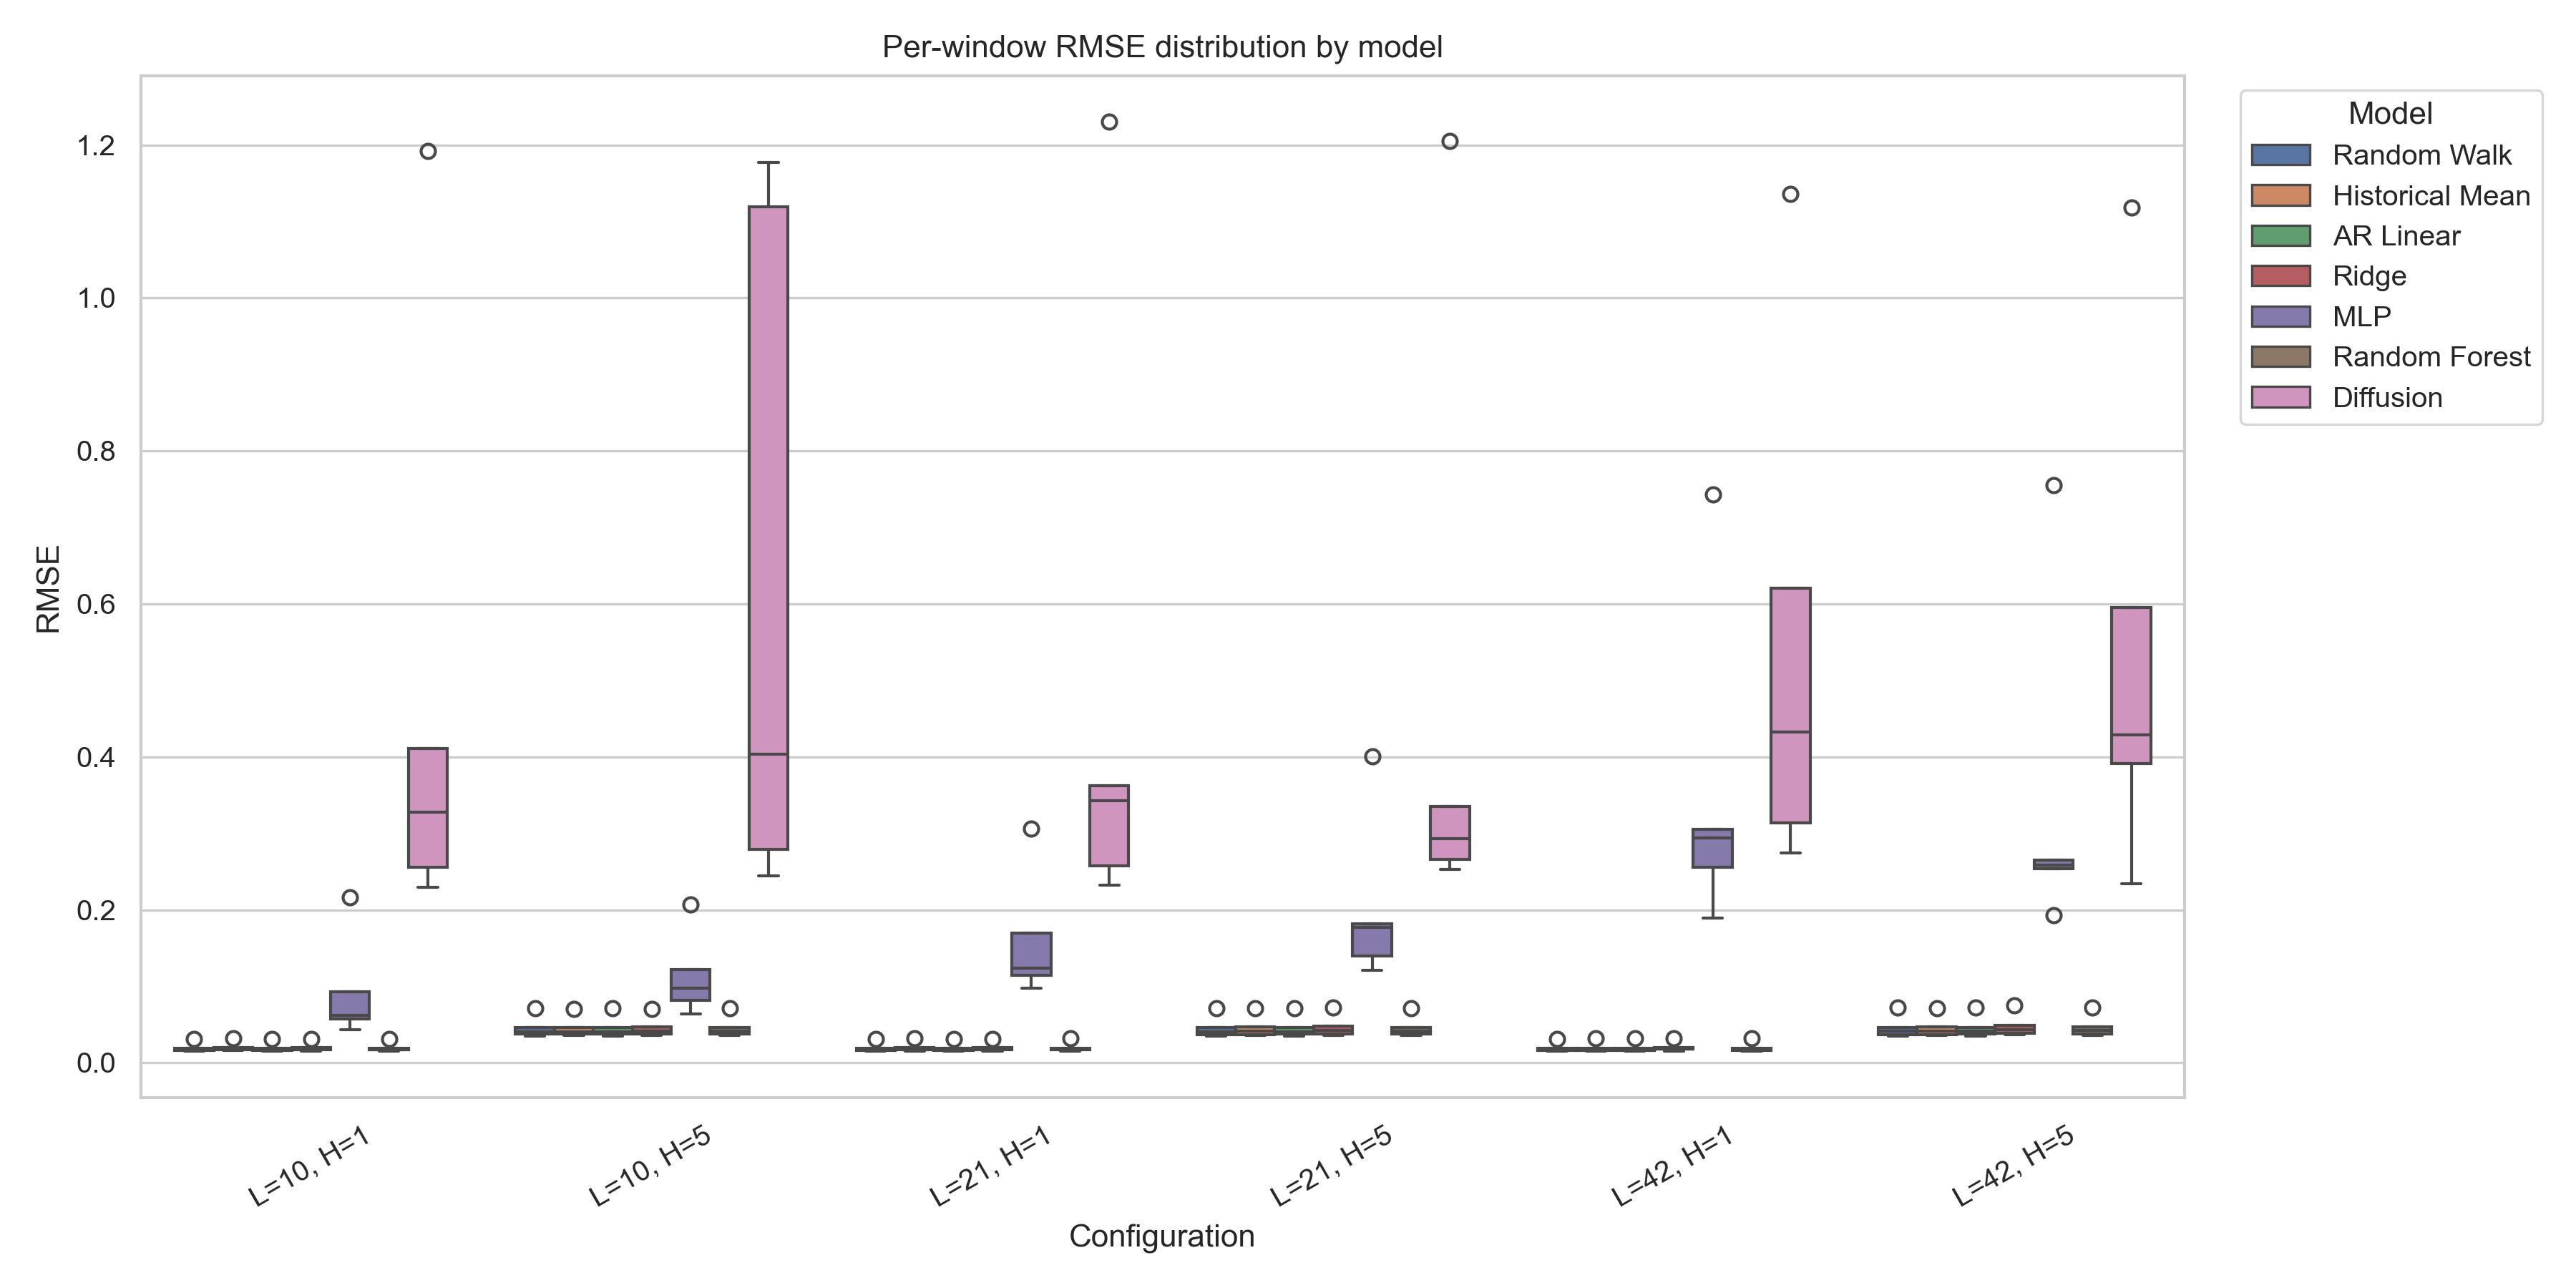
\includegraphics[width=0.96\linewidth]{../figures/generated/fig_rmse_by_model.png}
  \caption{Per-window RMSE distribution by model and configuration.}
  \label{fig:rmse}
\end{figure}

Random walk is the lowest-RMSE benchmark in all six \((L,H)\) configurations (\Cref{tab:rmse-by-config,tab:model-performance-summary,fig:rmse}). At \(H=1\), random-forest and linear-AR baselines are close to random walk in level terms but do not dominate consistently across lookback settings. At \(H=5\), historical mean and AR-linear models are again close to random walk, while more flexible ML models (MLP) degrade materially.

\subsection{Diffusion Model Performance}
Diffusion forecasts are worse than benchmark models in most configurations, but the absolute scale is close to the random-walk baseline: approximately 0.0201--0.0203 for \(H=1\) and 0.0464--0.0470 for \(H=5\) (\Cref{tab:rmse-by-config}).

\subsection{Formal Comparative Inference}
\begin{table}[!htbp]
\centering
\caption{Diebold-Mariano comparison versus random walk.}
\label{tab:dm-summary}
\begin{tabular}{lrr}
\toprule
Model & Mean DM statistic & Significant at 5\% \\
\midrule
AR Linear & -1.297 & 2 / 6 \\
Diffusion & -21.694 & 6 / 6 \\
Historical Mean & -1.594 & 3 / 6 \\
MLP & -11.505 & 6 / 6 \\
Random Forest & -2.002 & 3 / 6 \\
Ridge & -4.704 & 5 / 6 \\
\bottomrule
\end{tabular}
\caption*{\footnotesize Negative DM means the candidate model has higher loss than random walk.}
\end{table}


\begin{figure}[!htbp]
  \centering
  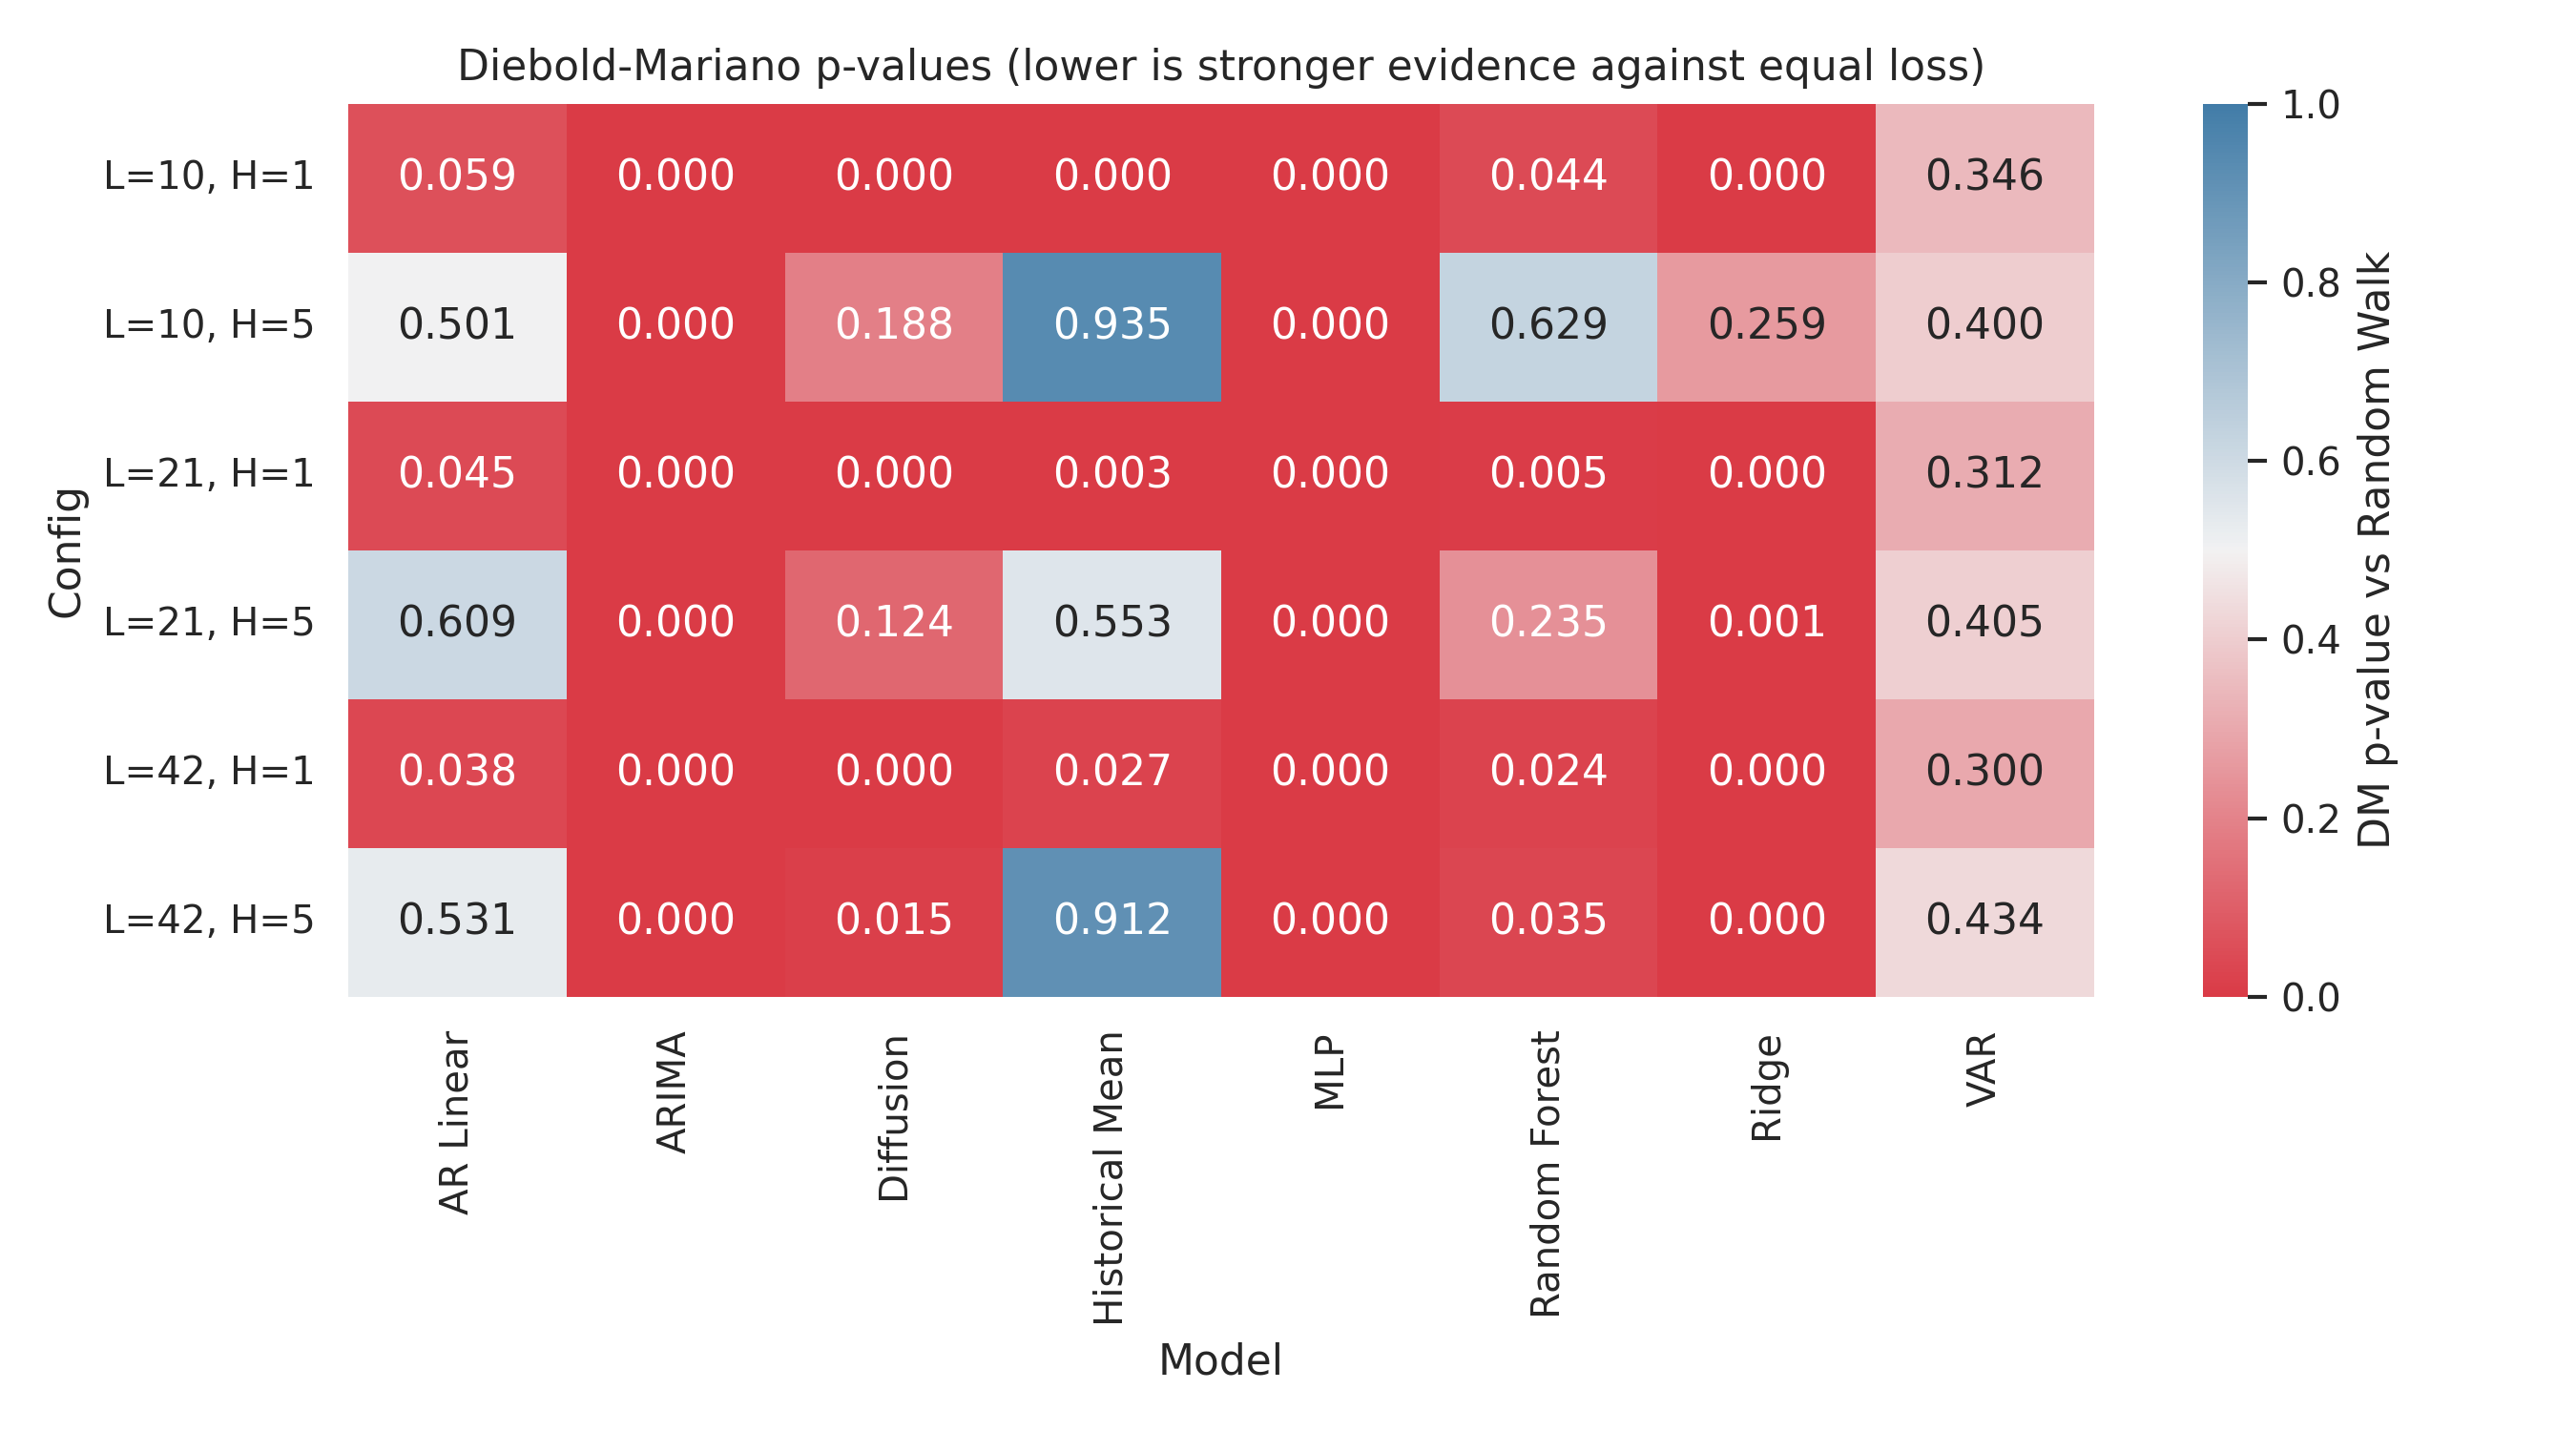
\includegraphics[width=0.86\linewidth]{../figures/generated/fig_dm_pvalue_heatmap.png}
  \caption{Diebold--Mariano p-values versus random walk.}
  \label{fig:dm-pvalue}
\end{figure}

\Cref{tab:dm-summary,fig:dm-pvalue} confirms that diffusion is significantly worse than random walk in four of six configurations under DM tests. At \(H=5\), diffusion is not significantly different from random walk for selected lookback settings, while ridge and MLP are typically inferior.

\subsection{XAI Findings}
\begin{figure}[!htbp]
  \centering
  \begin{subfigure}{0.49\linewidth}
    \centering
    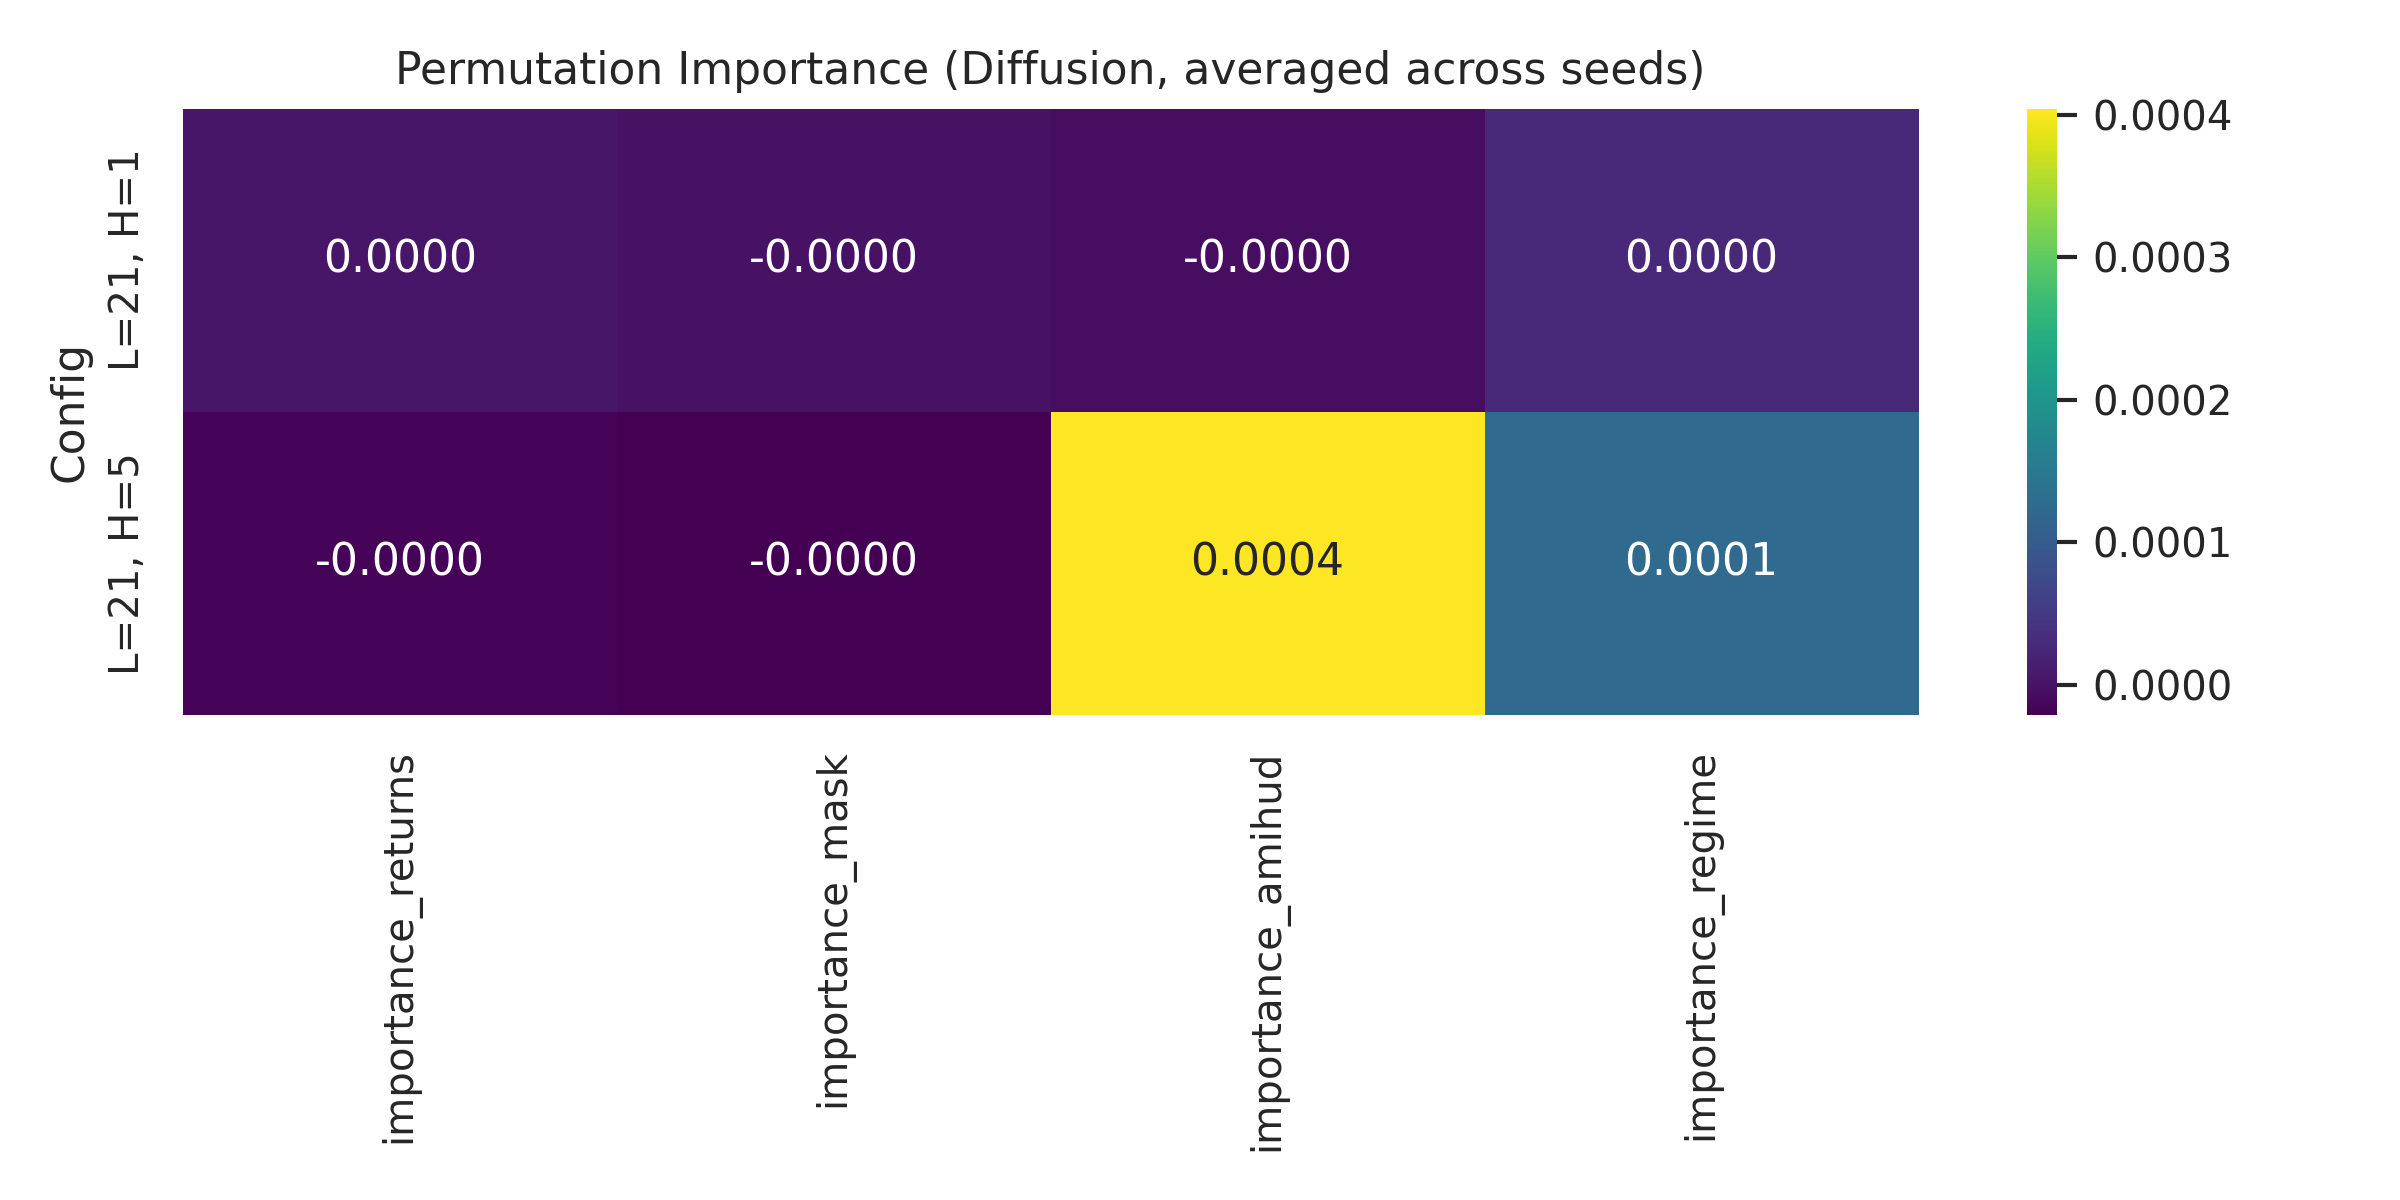
\includegraphics[width=\linewidth]{../figures/generated/fig_xai_importance_heatmap.png}
    \caption{Average permutation importance}
  \end{subfigure}
  \hfill
  \begin{subfigure}{0.49\linewidth}
    \centering
    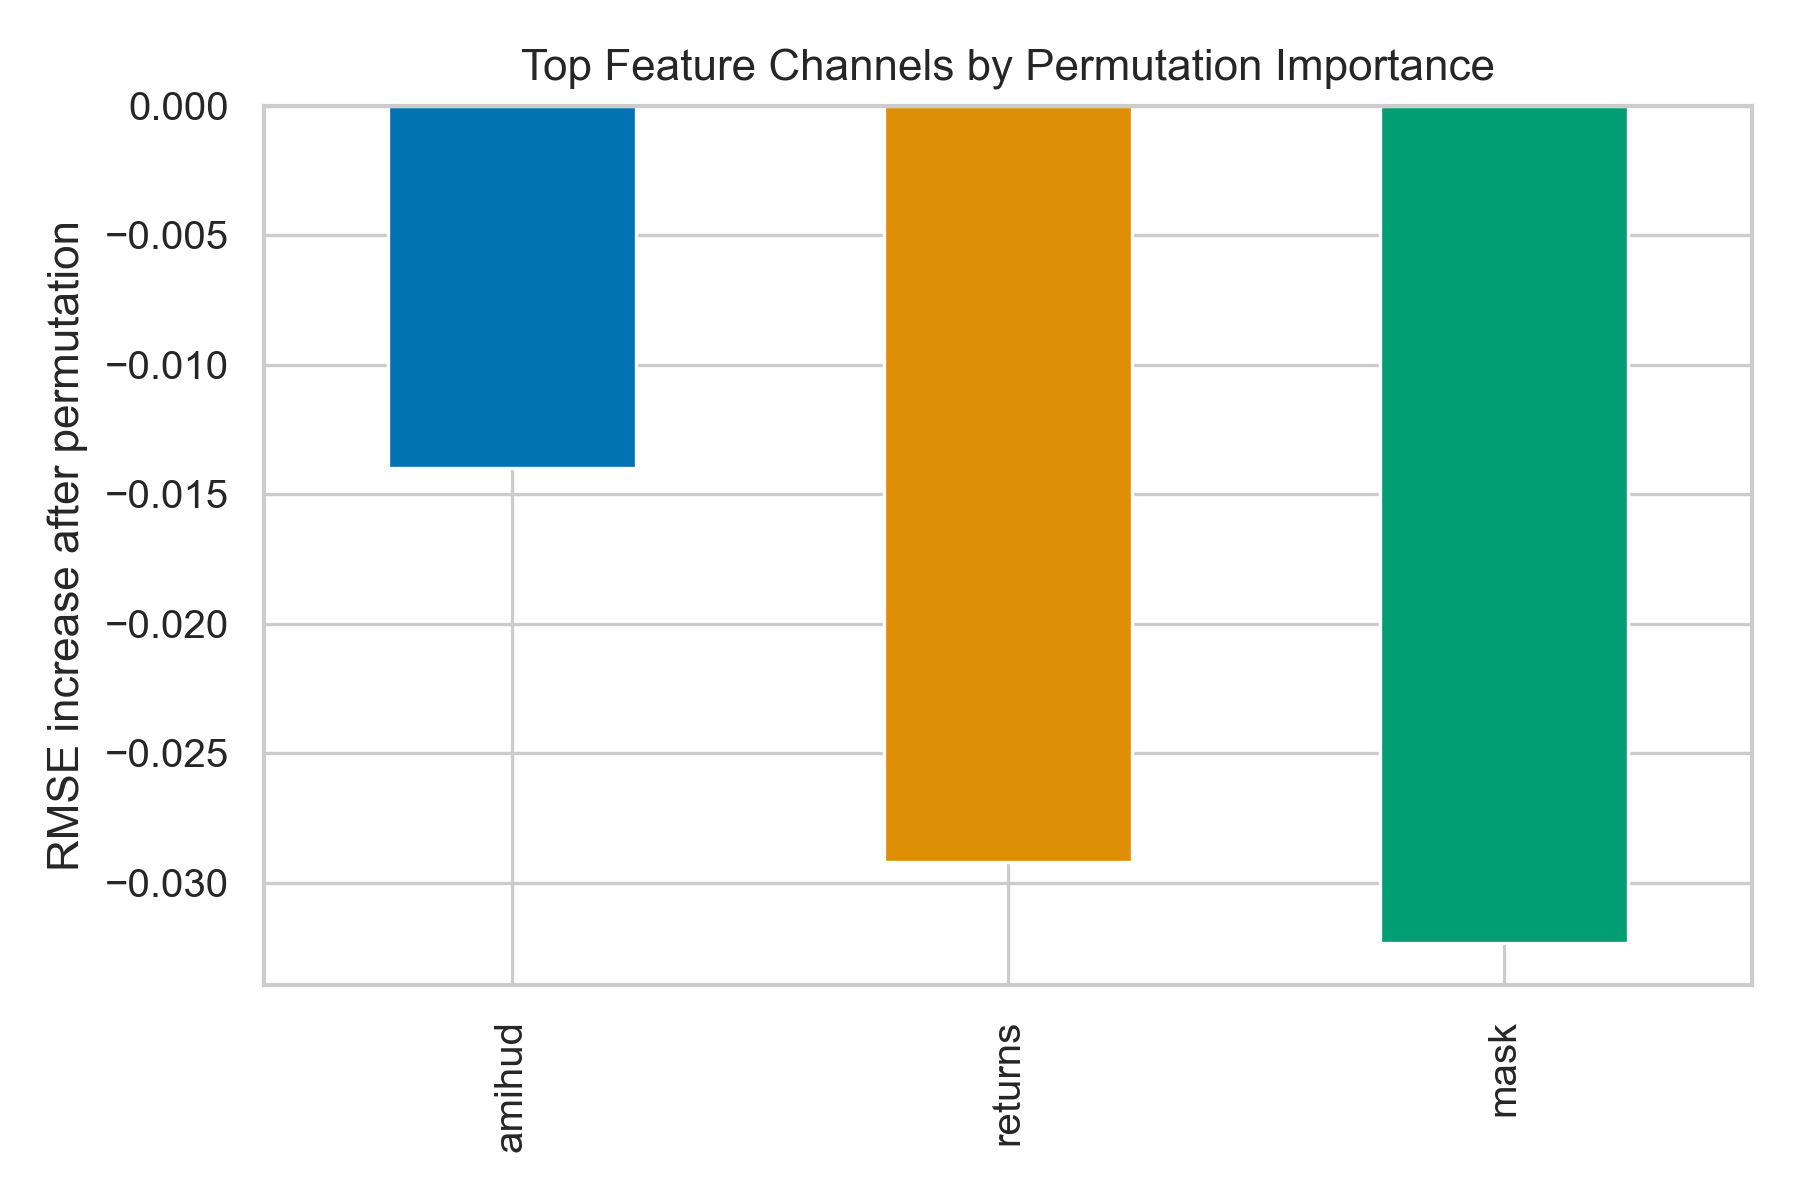
\includegraphics[width=\linewidth]{../figures/generated/fig_xai_top_features.png}
    \caption{Top feature channels}
  \end{subfigure}
  \caption{Diffusion model-reliance diagnostics from seed-level permutation analysis.}
  \label{fig:xai}
\end{figure}

\begin{table}[!htbp]
\centering
\caption{Permutation-importance max z-score sensitivity across diffusion seeds.}
\label{tab:xai-seed-sensitivity}
\begin{tabular}{lrrrr}
\toprule
L & H & Seed & Max z-score & Above 2.5 threshold \\
\midrule
21 & 1 & 0 & 1.170 & No \\
21 & 1 & 1 & 0.898 & No \\
21 & 1 & 2 & 1.189 & No \\
21 & 5 & 0 & 1.413 & No \\
21 & 5 & 1 & 1.414 & No \\
21 & 5 & 2 & 1.408 & No \\
\bottomrule
\end{tabular}
\end{table}

\begin{table}[!htbp]
\centering
\caption{XAI stability across seed pairs (Spearman correlation).}
\label{tab:xai-stability}
\begin{tabular}{lrrr}
\toprule
L & H & Seed pair & Spearman rho \\
\midrule
21 & 1 & 0-1 & 0.200 \\
21 & 1 & 0-2 & 0.400 \\
21 & 1 & 1-2 & -0.800 \\
21 & 5 & 0-1 & 0.400 \\
21 & 5 & 0-2 & 0.200 \\
21 & 5 & 1-2 & 0.800 \\
\bottomrule
\end{tabular}
\end{table}


XAI outputs are interpreted as model reliance only. \Cref{tab:xai-seed-sensitivity} shows no seed with max-\(z\) above 2.5, and \Cref{tab:xai-stability} shows unstable rank correlation across some seed pairs. Therefore, explanations are treated as fragile and non-structural.

\subsection{Robustness Checks and Sensitivity}
\begin{table}[!htbp]
\centering
\caption{Evaluation and leakage-control summary.}
\label{tab:robustness-summary}
\begin{tabular}{lr}
\toprule
Item & Value \\
\midrule
Evaluation windows & 5 \\
Total model-window evaluations & 330 \\
Leakage checks passed & True \\
Distinct benchmark models & 10 \\
MCS config rows & 6 \\
\bottomrule
\end{tabular}
\end{table}

\begin{table}[!htbp]
\centering
\caption{Diffusion sensitivity to feature-set ablations across seeds.}
\label{tab:diffusion-ablation}
\begin{tabular}{lrrrrr}
\toprule
L & H & Feature set & RMSE & MAE & RMSE std. \\
\midrule
21 & 1 & returns\_only & 0.02351 & 0.01599 & 0.00011 \\
21 & 1 & no\_illiquidity & 0.02352 & 0.01598 & 0.00010 \\
21 & 1 & full & 0.02375 & 0.01623 & 0.00023 \\
21 & 5 & full & 0.05334 & 0.03744 & 0.00005 \\
21 & 5 & returns\_only & 0.05344 & 0.03710 & 0.00008 \\
21 & 5 & no\_illiquidity & 0.05405 & 0.03759 & 0.00071 \\
\bottomrule
\end{tabular}
\end{table}

\begin{table}[!htbp]
\centering
\caption{Diffusion seed-level sensitivity by horizon and feature set.}
\label{tab:diffusion-seed-sensitivity}
\begin{tabular}{lrrrrr}
\toprule
L & H & Feature set & Seed & RMSE & MAE \\
\midrule
21 & 1 & full & 0 & 0.02375 & 0.01625 \\
21 & 1 & full & 1 & 0.02352 & 0.01599 \\
21 & 1 & full & 2 & 0.02398 & 0.01645 \\
21 & 1 & no\_illiquidity & 0 & 0.02360 & 0.01605 \\
21 & 1 & no\_illiquidity & 1 & 0.02356 & 0.01605 \\
21 & 1 & no\_illiquidity & 2 & 0.02341 & 0.01584 \\
21 & 1 & returns\_only & 0 & 0.02343 & 0.01592 \\
21 & 1 & returns\_only & 1 & 0.02364 & 0.01603 \\
21 & 1 & returns\_only & 2 & 0.02347 & 0.01603 \\
21 & 5 & full & 0 & 0.05340 & 0.03766 \\
21 & 5 & full & 1 & 0.05329 & 0.03732 \\
21 & 5 & full & 2 & 0.05334 & 0.03733 \\
21 & 5 & no\_illiquidity & 0 & 0.05355 & 0.03719 \\
21 & 5 & no\_illiquidity & 1 & 0.05374 & 0.03732 \\
21 & 5 & no\_illiquidity & 2 & 0.05487 & 0.03826 \\
21 & 5 & returns\_only & 0 & 0.05339 & 0.03702 \\
21 & 5 & returns\_only & 1 & 0.05353 & 0.03719 \\
21 & 5 & returns\_only & 2 & 0.05340 & 0.03710 \\
\bottomrule
\end{tabular}
\end{table}


\begin{figure}[!htbp]
  \centering
  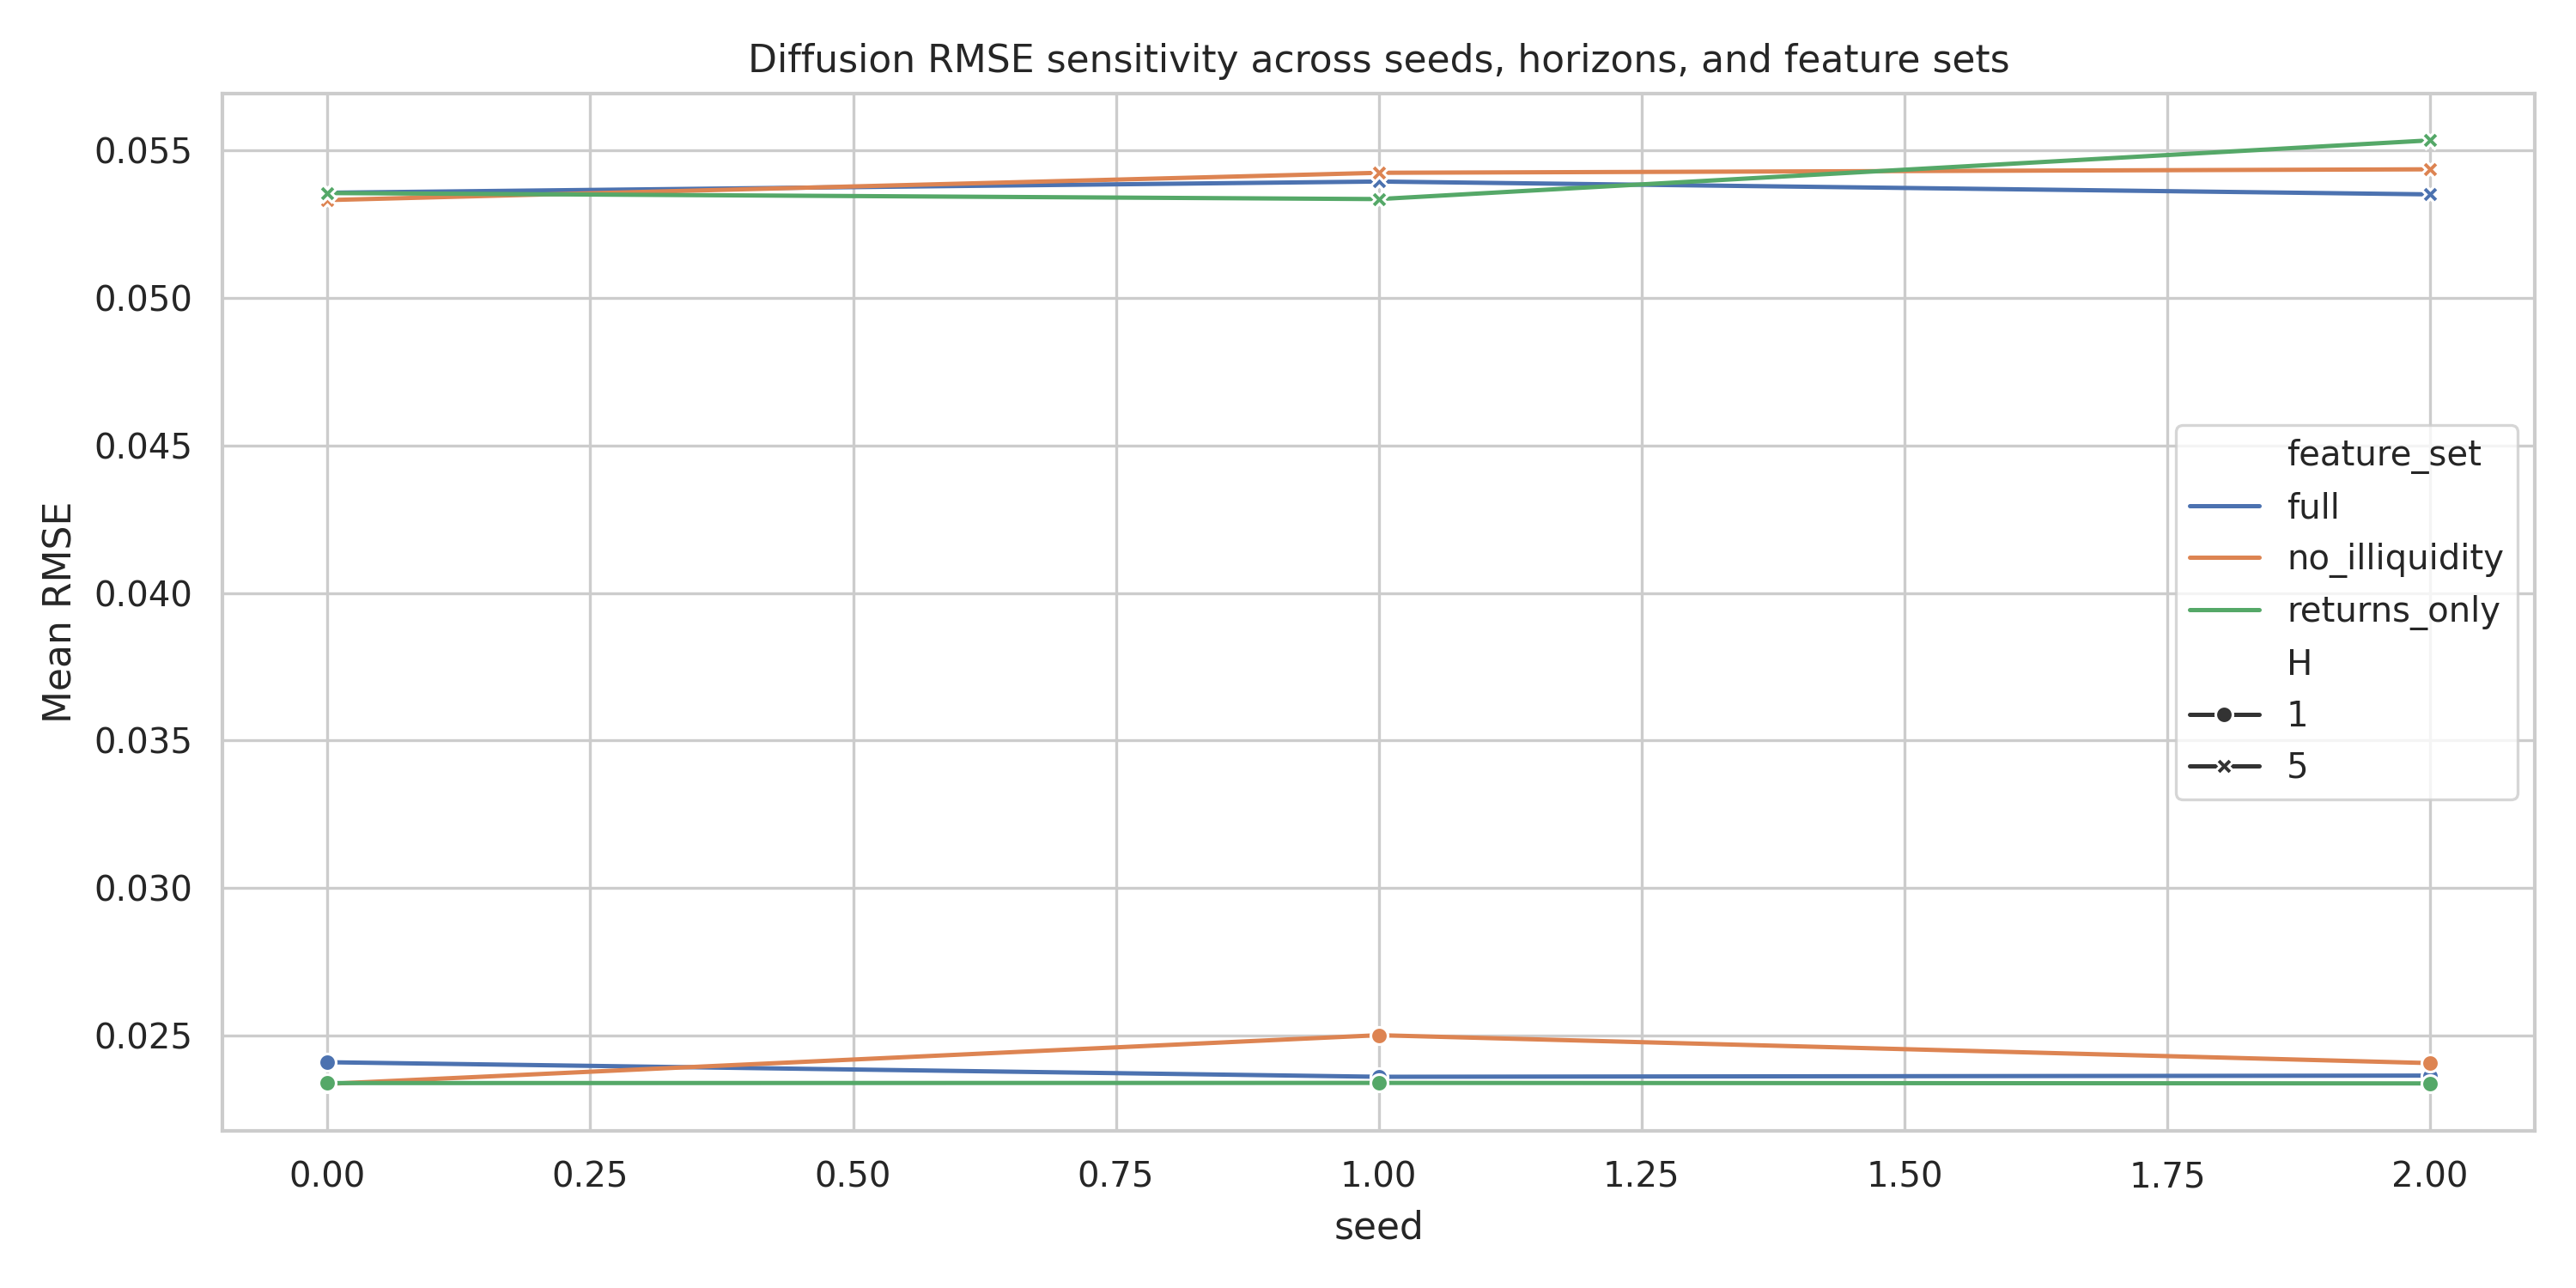
\includegraphics[width=0.84\linewidth]{../figures/generated/fig_diffusion_seed_sensitivity.png}
  \caption{Diffusion sensitivity across seeds, horizons, and feature sets.}
  \label{fig:diffusion-seed}
\end{figure}

Leakage assertions pass for all evaluation windows (\Cref{tab:robustness-summary}). Diffusion ablations in \Cref{tab:diffusion-ablation,tab:diffusion-seed-sensitivity,fig:diffusion-seed} indicate meaningful sensitivity to feature design and seed choice, with no robust improvement over benchmark models.

\subsection{EMH Interpretation}
Under a benchmark-relative predictability interpretation of weak-form EMH, the present evidence is consistent with limited extractable out-of-sample predictive gains beyond simple benchmarks in this dataset and design. This is a predictive, not structural, statement: the analysis does not establish exploitable abnormal profits, causal inefficiency mechanisms, or post-cost economic significance.
